\section{Analysis and Results}
\label{sec:description_3}

%\subsection{$2$ Player Game}
%\label{subsec:2playergame}

\subsection{$3$ Player Game}
\label{subsec:3playergame}

\subsubsection{The captain proposes: $(99, 0, 1)$}
\label{subsubsec:3playergame99}

The outcome $CDC$ with a proposal of $(\alpha_{1}, \alpha_{2}, \alpha_{3}) =(99, 0, 1)$ would represent the Nash Equilibrium of the classic Pirate Game (for $3$ players). 

When the players chose at least $2$ operators $Cooperate$ on the initial proposal the game ends right away, the disentangle operator $\mathcal{J}^{\dagger}$ is applied, and the payoff functionals are calculated given the final state. The final state will be calculated as in Equation \ref{eq:piratas_final_move2_99anal}. 

The Tables \ref{tab:3playerCCC99}, \ref{tab:3playerCCD99}, \ref{tab:3playerCDC99}, and \ref{tab:3playerDCC99}, in the Apendix \ref{ap:d}
,present the results for the sittuation described above.

In the Table \ref{repro:1} we find a reproduction of Table \ref{tab:3playerCCC99}, where the $3$ players choose to use the cooperate strategy. We can see that the parameter $\gamma$ has no effect on the final result. This happens because no player choose to change her qubit. 

In Tables \ref{tab:3playerCCD99}, \ref{tab:3playerCDC99}, and \ref{tab:3playerDCC99} we can see a pattern on the probability distributions of measuring a determined state. The Table \ref{repro:2} reproduces the results of Table \ref{tab:3playerCDC99}. 

The state corresponding to the operators chosen by the players and the state where all qubits are flipped (for example $CDC$ and $DCD$), vary with $\gamma$, such that $P(CDC)= 1 - P(DCD)$. The state where the qubits are flipped ($DCD$ for example), approximates a normal distribution (when we vary $\gamma$). The peak for this distribution happens when the initial system is maximally entangled.

For $\gamma = 0 + k \pi, k \in \{0,1\}$ we are rendered with the classical situation, this means the proposal suggested by the captain will be enforced exactly as she stated. When $\gamma = \frac{\pi}{2}$ we are before a symmetric outcome where player 1 would die and player 2 would approve her proposal and get the $100$ coins.


\begin{equation}
\label{eq:piratas_final_move2_99anal}
\vert\psi_{fin}\rangle= \mathcal{J}^{\dagger}\vert\psi_{1}\rangle
\end{equation}



 
\begin{table}
\begin{center}
\begin{tabular}{cc}
  a)\putindeepbox[7pt]{\includegraphics[scale=0.46]{3Accepted99/CCC.PNG}}
    & a1)\putindeepbox[7pt]{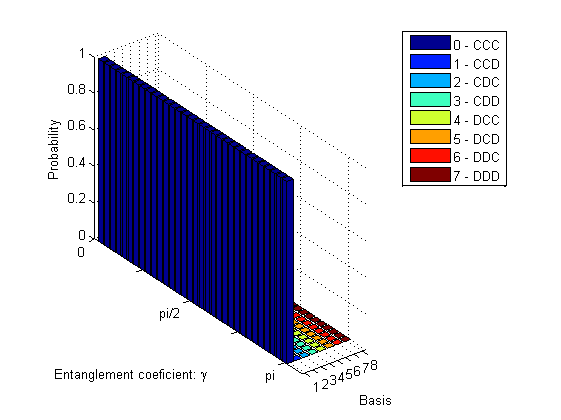
\includegraphics[scale=0.46]{3Accepted99/CCC_1.PNG}} \\
\end{tabular}
\caption{a) Expected utility for $3$ players, where the players will use the $(Cooperate, Cooperate, Cooperate)$ operators. The initial proposal is $(\alpha_{1}, \alpha_{2}, \alpha_{3}) =(99, 0, 1)$. a1) Probability distribution of the final state depending on the entanglement coefficient $\gamma$.  Reproduction from Table \ref{tab:3playerCCC99}}
\label{repro:1}
\end{center}
 \end{table}

\begin{table}
\begin{center}
\begin{tabular}{cc}
  b)\putindeepbox[7pt]{\includegraphics[scale=0.46]{3Accepted99/CDC.PNG}}
    & b1)\putindeepbox[7pt]{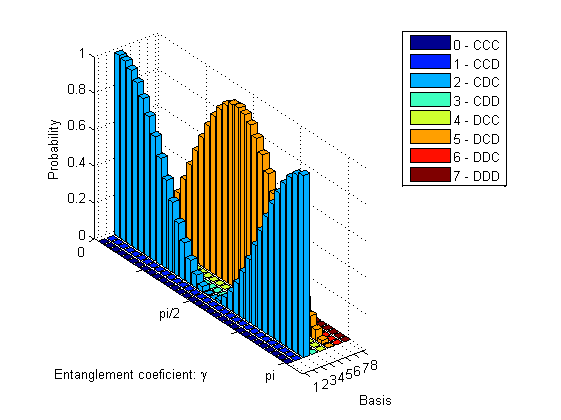
\includegraphics[scale=0.46]{3Accepted99/CDC_1.PNG}} \\
\end{tabular}
\caption{b) Expected utility for $3$ players, where the players will use the $(Cooperate, Defect, Cooperate)$ operators. b1) Probability distribution of the final state depending on the entanglement coefficient $\gamma$.  Reproduction from Table \ref{tab:3playerCDC99}.}
\label{repro:2}
\end{center}
 \end{table}

When the first proposal is rejected (more than $1$ player chooses to $Defect$), the second round ensues. We calculate the final state for these states with Equation \ref{eq:piratas_final_move2_99anal1}. 


\begin{equation}
\label{eq:piratas_final_move2_99anal1}
\vert\psi_{fin}\rangle= \mathcal{J}^{\dagger}\vert\psi_{2}\rangle
\end{equation}

In a classical game the best response for player $1$ is to cooperate. In this quantum version depending of the parameter $\gamma$, the strategy that produces the most favourable outcome changes. However if the first proposal is rejected and the player $1$ voted in favour (using the $C$ operator), we get to a final subgame where the parameter $\gamma$ won't influence the expected utility; the results for this can be consulted on Apendix \ref{ap:d}, Section \ref{ap:d:CDD99}. This happens due to a design rule in the way we calculate our expected utility for each player, but the parameter $\gamma$ affects the probability of the system being measured in a determined state, as in Table \ref{repro:3}.

 \begin{table}
\begin{center}
\begin{tabular}{cc}
  c)\putindeepbox[7pt]{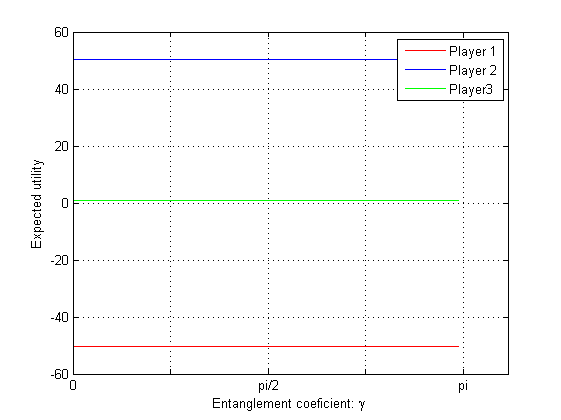
\includegraphics[scale=0.46]{3Rejected99/CDD_CD.PNG}}
    & c1)\putindeepbox[7pt]{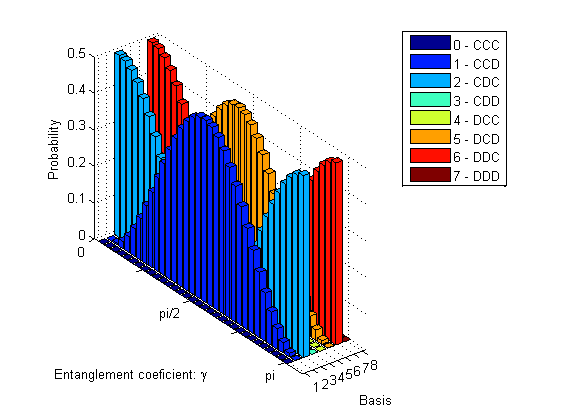
\includegraphics[scale=0.46]{3Rejected99/CDD_CD1.PNG}} \\
\end{tabular}
\caption{Expected utility for $3$ players, where the players will use the $(Cooperate , Defect, Defect)$ operators in the first round of the game; in the second round player 2 and player 3 will play $(CD)$.}
\label{repro:3}
\end{center}
 \end{table}

If in the quantum game the player $1$ decides to defect $D$ and the proposal is rejected we get $4$ different probability distributions that are permuted given the players chosen operators. For example in Tables \ref{tab:3playerDCD_DC99}, 
\ref{tab:3playerDDC_CD99}, and \ref{tab:3playerDDD_CC99} (in Apendix \ref{ap:d}): the player $2$ has assumes the strategy $\tau_{2}=CD$ in Table \ref{tab:3playerDCD_DC99}, in Table \ref{tab:3playerDDC_CD99} her stategy is $\tau_{2}=DC$, as the multiplication by a identity matrix is comutative in both cases we applied the same operation to player $2$ qubit. This result happens because the players are manipilating their qubits with permutation operators.

\subsubsection{The captain proposes: $(100, 0, 0)$}
\label{subsubsec:3playergame100}

Suppose captain is greedy and proposes to get the 100 coins. In the classical Pirate Game this would pose a conflict with his self-preserving needs. 
A pertinent question would be if this Quantum Model of the Pirate Game would allow the first captain to approve an allocation proposal. The initial proposal will be accepted if there is at least $2$ players play $\mathcal{U}_{i}=C$ in a round. In order to answer our question we must analyse the expected utilities for all players when the initial proposal is accepted.

 Our final state will be calculated as in Equation \ref{eq:piratas_final_move2_99anal}.

\begin{table}
\begin{center}
\begin{tabular}{c}
  a)\putindeepbox[7pt]{\includegraphics[scale=0.72]{3Accepted100/CCC.PNG}}
\end{tabular}
\caption{a) Expected utility for $3$ players, where the players will use the $(Cooperate, Cooperate, Cooperate)$ operators. The initial proposal is $(\alpha_{1}, \alpha_{2}, \alpha_{3}) =(100, 0, 0)$. }
\label{tab:3playerCCC100}
\end{center}
 \end{table}

\begin{table}
\begin{center}
\begin{tabular}{c}
  b)\putindeepbox[7pt]{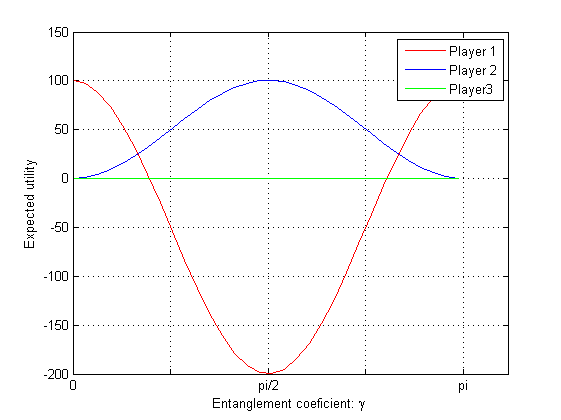
\includegraphics[scale=0.72]{3Accepted100/CCD.PNG}}
\end{tabular}
\caption{b) Expected utility for $3$ players, where the players will use the $(Cooperate, Cooperate, Defect)$ operators. }
\label{tab:3playerCCD100}
\end{center}
 \end{table}

\begin{table}
\begin{center}
\begin{tabular}{c}
  c)\putindeepbox[7pt]{\includegraphics[scale=0.72]{3Accepted100/CDC.PNG}}
   
\end{tabular}
\caption{c) Expected utility for $3$ players, where the players will use the $(Cooperate, Defect, Cooperate)$ operators.}
\label{tab:3playerCDC100}
\end{center}
 \end{table}

\begin{table}
\begin{center}
\begin{tabular}{cc}
  d)\putindeepbox[7pt]{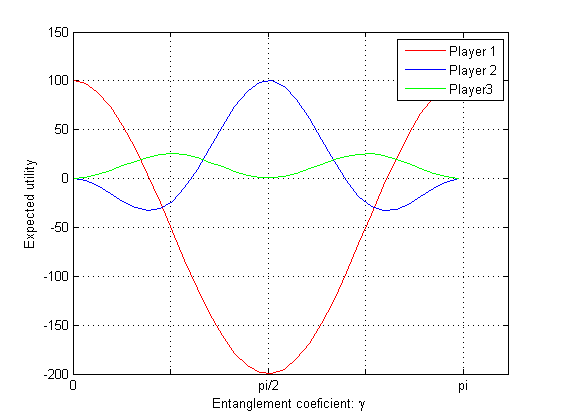
\includegraphics[scale=0.72]{3Accepted100/DCC.PNG}}
\end{tabular}
\caption{d) Expected utility for $3$ players, where the players will use the $(Defect, Cooperate, Cooperate)$ operators. }
\label{tab:3playerDCC100}
\end{center}
 \end{table}




